\section{Sensitivity and robustness}
\label{sec:sensitivity}

\paragraph{Tornado analysis of the investment decision.} For each of nine parameters we re-optimised the
normal-year investment problem (500~MEUR, representative weeks) at a low and a high value
(Fig.~\ref{fig:sensitivity}a). The optimal annualised system cost is most sensitive to the following
parameters, in decreasing order of effect:
\begin{itemize}
\item drought severity: $+213.5$~MEUR/yr at $d=0.3$;
\item demand ($\pm10\%$): $-74.3$/$+68.4$~MEUR/yr;
\item the export/import price ratio: $+30.0$/$-18.8$~MEUR/yr at 0.75/0.95;
\item PV capex ($\pm30\%$): $-34.7$/$+19.1$~MEUR/yr;
\item the import price ($\pm30\%$): $+13.3$/$-13.3$~MEUR/yr;
\item the discount rate (4\%/10\%): $-10.9$/$+12.1$~MEUR/yr.
\end{itemize}
The \emph{technology choice}, all PV, is unchanged across every case. Only the PV amount responds, to its own
capex: 899~MW at $\times0.7$ and 484~MW at $\times1.3$. The budget binds in both cases. VOLL and battery capex
have no effect because no shortage occurs and no battery is chosen. Interconnector capacity between 600 and
1{,}200~MW moves cost by less than 3~MEUR/yr in a normal year. The importance of interconnection appears only
under joint stress (Experiments F, G and J).

\paragraph{Drought severity sweep.} Increasing the inflow reduction $d$ from 0 to 0.6 in steps of 0.05, with
the existing fleet, raises imports almost linearly: from 2.0 to 4.9~TWh/yr with full transfer availability,
while annual cost rises from 41 to 481~MEUR (Fig.~\ref{fig:imports}a). No shortage occurs at any severity with
full availability. With 50\% availability the system copes up to $d=0.4$, and unserved energy then jumps to
341~GWh at $d=0.5$ and 956~GWh at $d=0.6$ (Fig.~\ref{fig:imports}b). The reliability boundary of the system
therefore lies in the joint space of drought severity and import availability.

\paragraph{Battery value across drought and import stress.} With import availability at 60\%, the net benefit
of a 4-hour battery (operating saving minus annualised cost) is negative up to drought severity $d=0.4$:
between $-10$ and $-97$~MEUR/yr for 400--3{,}200~MWh (Fig.~\ref{fig:sensitivity}b). It turns strongly positive
at $d=0.6$, where shortage occurs: $+248$ to $+332$~MEUR/yr. There the battery reduces unserved energy from 281
to between 228 and 192~GWh, and each avoided MWh is valued at VOLL. Batteries in this system are therefore
\emph{reliability} assets under joint drought and import stress, not arbitrage assets. Their economic case
depends on the probability of such joint events and on the VOLL assumed for them. This is the case where
the VOLL assumption matters most.

\paragraph{Temporal resolution.} The operating saving from a 400~MW / 1{,}600~MWh battery is 9.8, 8.8, 7.0 and
1.3~MEUR/yr at 1-, 2-, 3- and 6-hour time steps, and its cycling falls from 401 to 111 equivalent full cycles
(Fig.~\ref{fig:resolution}). Six-hourly steps remove 87\% of the battery's arbitrage value. This explains why the
first, 6-hourly version of our stochastic model selected no storage, and why the investment studies use hourly
representative weeks.

\begin{figure}[htbp]
\centering
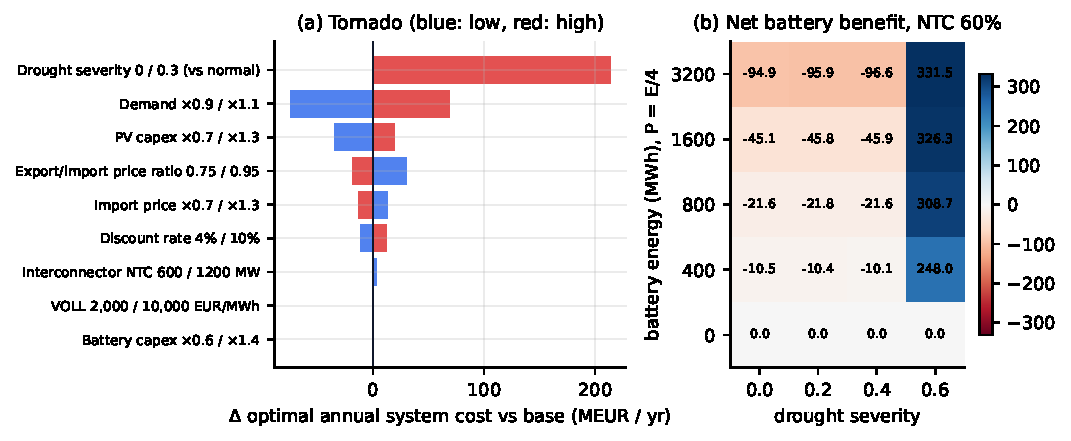
\includegraphics[width=\textwidth]{fig10_sensitivity.pdf}
\caption{(a) Change in the optimal annualised system cost when each parameter is set to its low (blue) or high
(red) value, with investment re-optimised each time. (b) Net annual benefit (MEUR/yr) of a 4-hour battery as a
function of drought severity and battery size, with import availability 60\%.}
\label{fig:sensitivity}
\end{figure}

\begin{figure}[htbp]
\centering
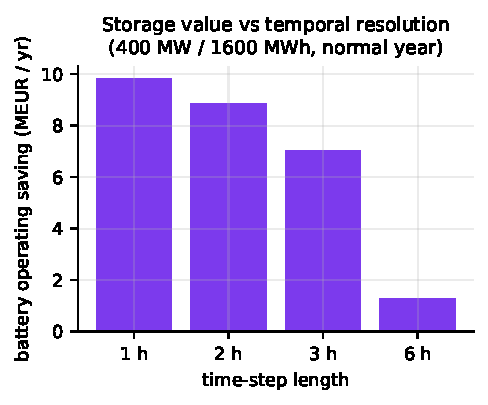
\includegraphics[width=0.5\textwidth]{fig12_resolution.pdf}
\caption{Operating value of a 400~MW / 1{,}600~MWh battery in the normal year as a function of the time-step
length.}
\label{fig:resolution}
\end{figure}
